\documentclass[11pt,a4paper]{article}

\usepackage[utf8]{inputenc}
\usepackage[spanish,es-tabla]{babel}
\usepackage[margin=2.5cm]{geometry}
\usepackage{graphicx}
\usepackage{booktabs}
\usepackage{amsmath}
\usepackage{siunitx}
\usepackage{float}
\usepackage[hidelinks]{hyperref}
\usepackage{caption}
\captionsetup{font=small,labelfont=bf}

\graphicspath{{../data/outputs/figs/}}
\newcommand{\tab}[1]{\input{../data/outputs/tabs/#1}}

\title{\textbf{Accesibilidad vial a servicios de emergencia resolutivos\\
en Lambayeque, Apur\'imac y Amazonas}\\[0.3em]
\large An\'alisis geoespacial, m\'etricas de cobertura y desigualdad}
\author{Karelys S. Collazos \\
\small Data Science with Python --- HW\_02\_202602 --- \texttt{d2cml-ai/Data-Science-Python} \#186}
\date{\today}

\begin{document}
\maketitle

\begin{abstract}
\noindent
La \emph{hora dorada} en medicina de emergencia postula que la probabilidad de
supervivencia cae de forma marcada si el paciente no recibe atenci\'on
resolutiva en los primeros 60 minutos. Este trabajo estima, para
\num{8781} centros poblados de tres departamentos que representan la costa
(Lambayeque), la sierra (Apur\'imac) y la selva (Amazonas), el tiempo de viaje
\emph{por carretera} hasta el establecimiento de salud resolutivo m\'as cercano
(categor\'ia II-1 o superior). Se construye una matriz origen--destino de
\num{342} mil pares con OSRM, se ponderan los indicadores por poblaci\'on del
Censo 2017 y se analiza la cobertura, la desigualdad (Gini) y su relaci\'on con
altitud y pobreza distrital. \textbf{Resultado principal:} cerca del
\SI{24}{\percent} de la poblaci\'on queda fuera de la hora dorada, con un Gini de
acceso de \num{0.62} y un gradiente claro con la pobreza: el cuartil de
distritos m\'as pobres tarda del orden de seis veces m\'as que el menos pobre.
\end{abstract}

\section{Introducci\'on y planteamiento del problema}

La distancia en l\'inea recta a un hospital subestima sistem\'aticamente el
tiempo real de traslado, sobre todo en zonas andinas y amaz\'onicas donde la red
vial es sinuosa o escasa. La pregunta de investigaci\'on es: \emph{¿qu\'e
fracci\'on de la poblaci\'on de cada regi\'on natural puede alcanzar un
establecimiento resolutivo dentro de la hora dorada, y c\'omo se distribuye esa
carencia entre territorios urbanos y rurales, de mayor y menor altitud, y de
mayor y menor pobreza?}

Objetivos: (i) construir datasets validados de oferta (establecimientos II-1+) y
demanda (centros poblados con poblaci\'on); (ii) calcular tiempos de viaje
viales; (iii) derivar indicadores de cobertura y desigualdad ponderados por
poblaci\'on; (iv) identificar los distritos con mayor brecha.

\section{Datos}

\subsection{Fuentes}
\begin{itemize}
  \item \textbf{Oferta.} RENIPRESS (SUSALUD), padr\'on de agosto de 2026.
        Se retienen los establecimientos \textsc{activo}s de categor\'ia
        II-1, II-2, II-E, III-1, III-2 o III-E.
  \item \textbf{Demanda.} Centros poblados del Censo 2017 (INEI, distribuci\'on
        geogpsperu) con poblaci\'on, altitud, categor\'ia y coordenadas.
  \item \textbf{L\'imites distritales.} Cartograf\'ia distrital (l\'imites INEI).
  \item \textbf{Contexto.} Pobreza monetaria e IDH distrital
        (INEI\,/\,PNUD, v\'ia \texttt{ubigeo-peru-aumentado}).
  \item \textbf{Red vial.} OpenStreetMap, servida por OSRM.
\end{itemize}

\subsection{Validaci\'on y control de calidad}
Se aplicaron reglas autom\'aticas de detecci\'on sin eliminar registros: cada
fila conserva sus banderas \texttt{qc\_*} y se excluye del an\'alisis solo si
falla una regla cr\'itica. Las Tablas~\ref{tab:calidad-oferta}
y~\ref{tab:calidad-demanda} resumen los hallazgos.

\tab{tab_calidad_oferta.tex}
\tab{tab_calidad_demanda.tex}

Hallazgos destacados: una fracci\'on relevante de establecimientos figura sin
coordenadas o con categor\'ia no v\'alida (\texttt{"0"}); se detectaron
duplicados espaciales dentro de un mismo distrito. En la demanda, la capa de
centros poblados de un departamento (Tumbes, descartado del estudio) lleg\'o sin
c\'odigo ni poblaci\'on, lo que motiv\'o el cambio a Lambayeque; para Amazonas y
Apur\'imac la cobertura de poblaci\'on es del \SI{100}{\percent}.

\section{Metodolog\'ia}

\subsection{Ruteo y matriz origen--destino}
Cada centro poblado y cada establecimiento se asocian a la red vial de OSM. Con
el servicio \texttt{/table} de OSRM se calcula, por lotes y con cach\'e SQLite
reanudable, la duraci\'on y la distancia de conducci\'on entre los \num{8781}
or\'igenes y los establecimientos resolutivos. El \SI{100}{\percent} de los pares
obtuvo ruta real; para pares sin ruta se prev\'e el \emph{fallback}
$t = d_{\text{haversine}}\cdot \kappa / v$ con factor de rodeo $\kappa=1{,}3$.
El perfil \emph{caminando} se estima a partir de la distancia vial a
\SI{4.5}{\km\per\hour} (el servidor p\'ublico de OSRM no expone perfil peatonal),
y se reporta como cota comparativa.

Se consider\'o un motor alternativo con grafo local (\texttt{osmnx} +
\texttt{networkx}); se descart\'o porque la descarga del grafo de tres
departamentos desde Overpass supera reiteradamente el tiempo de espera. El
c\'odigo de ese motor permanece disponible.

\subsection{M\'etricas}
Para cada centro poblado $i$ se toma el tiempo m\'inimo
$t_i=\min_j t_{ij}$ al conjunto de establecimientos $j$. Con poblaci\'on $w_i$:
\begin{itemize}
  \item \textbf{Cobertura} por bandas: \% de $\sum w_i$ con $t_i\le\{30,60,120\}$ min.
  \item \textbf{Tiempo medio ponderado} $\bar t = \sum w_i t_i / \sum w_i$.
  \item \textbf{Desigualdad}: Gini ponderado del vector $\{t_i\}$,
  \begin{equation}
    G = 1 - \frac{\sum_{k} (C_k + C_{k-1})\,(W_k - W_{k-1})}{C_n},\quad
    C_k = \!\!\sum_{m\le k}\! w_m t_m,\ \ W_k=\!\!\sum_{m\le k}\! w_m,
  \end{equation}
  con los $i$ ordenados por $t_i$ ascendente.
  \item \textbf{Cruces}: $\bar t$ por \'ambito urbano/rural, por tercil de
        altitud y por cuartil de pobreza distrital; correlaci\'on de $t_i$ con
        \% de pobreza e IDH.
\end{itemize}
La poblaci\'on de los centros poblados sin dato (caso Tumbes, no incluido) se
imputar\'ia repartiendo el total distrital seg\'un la categor\'ia del centro
poblado; en el \'ambito final la imputaci\'on afecta al
\SI{0}{\percent} de la poblaci\'on.

\section{Resultados}

\begin{figure}[H]
  \centering
  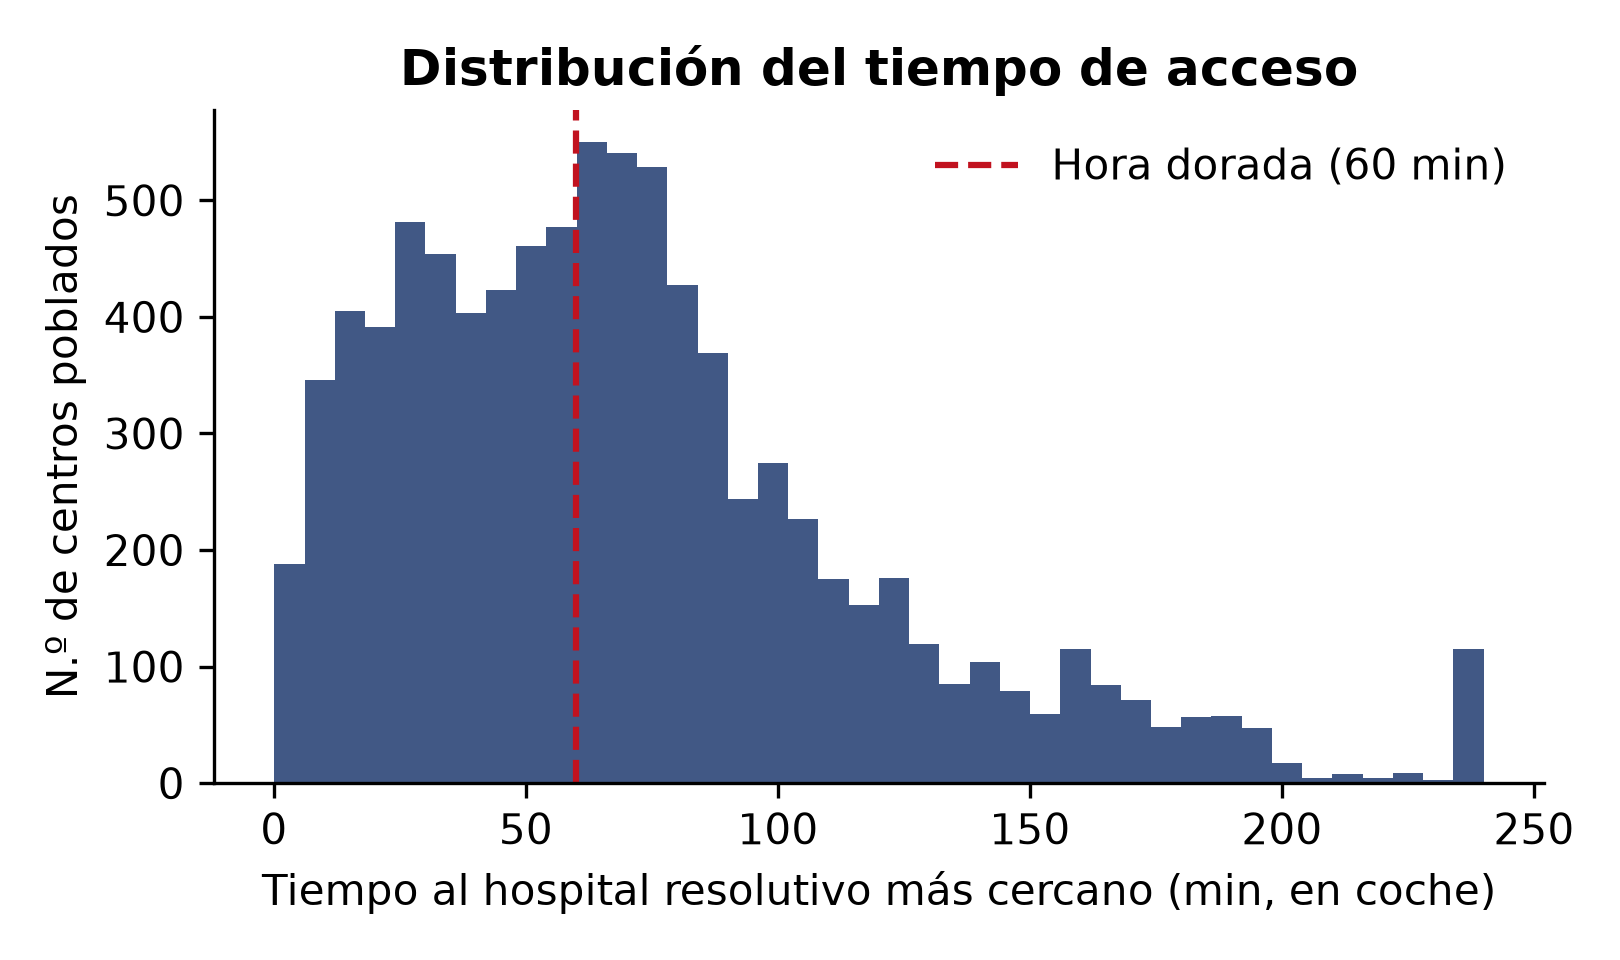
\includegraphics[width=0.72\linewidth]{fig_hist_acceso.png}
  \caption{Distribuci\'on del tiempo de acceso al hospital resolutivo m\'as
  cercano (conducci\'on). La l\'inea marca la hora dorada.}
  \label{fig:hist}
\end{figure}

\begin{figure}[H]
  \centering
  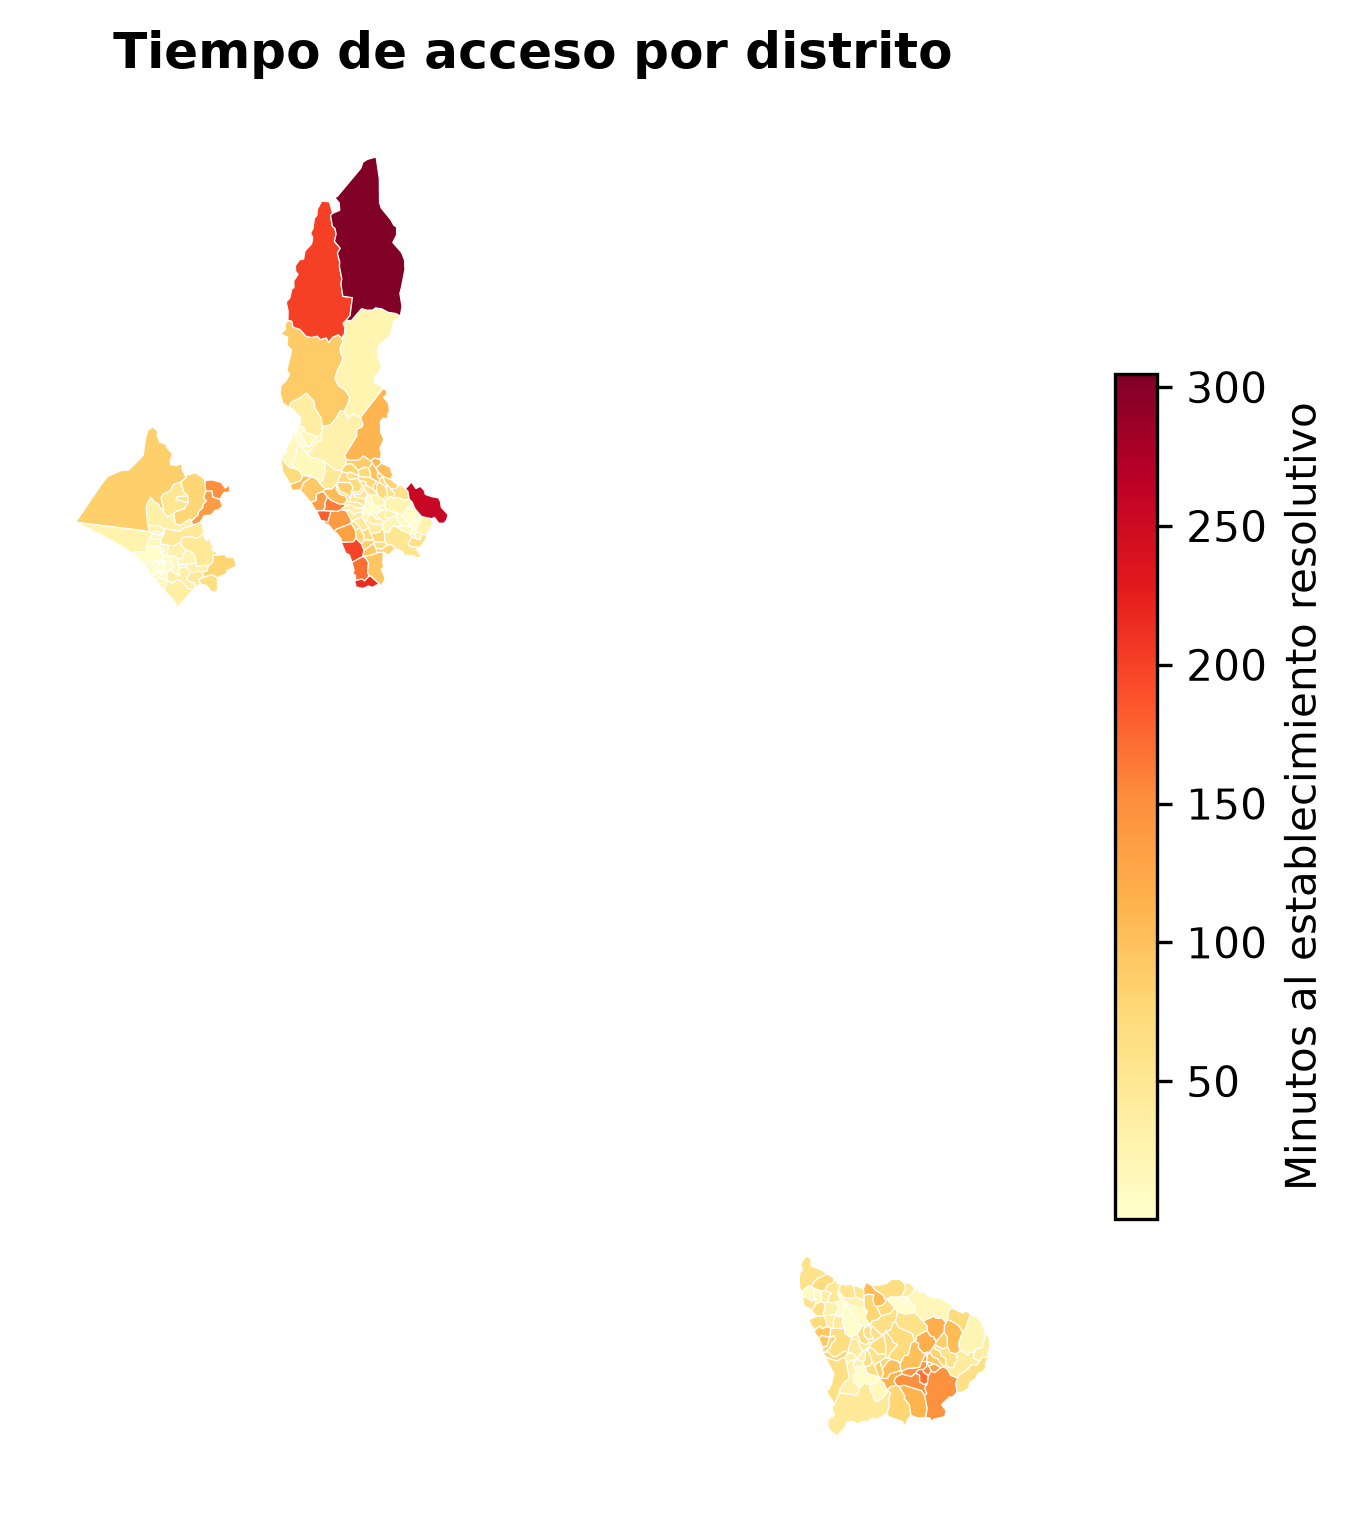
\includegraphics[width=0.62\linewidth]{fig_choropleth.png}
  \caption{Tiempo de acceso ponderado por poblaci\'on, por distrito.}
  \label{fig:choropleth}
\end{figure}

\begin{figure}[H]
  \centering
  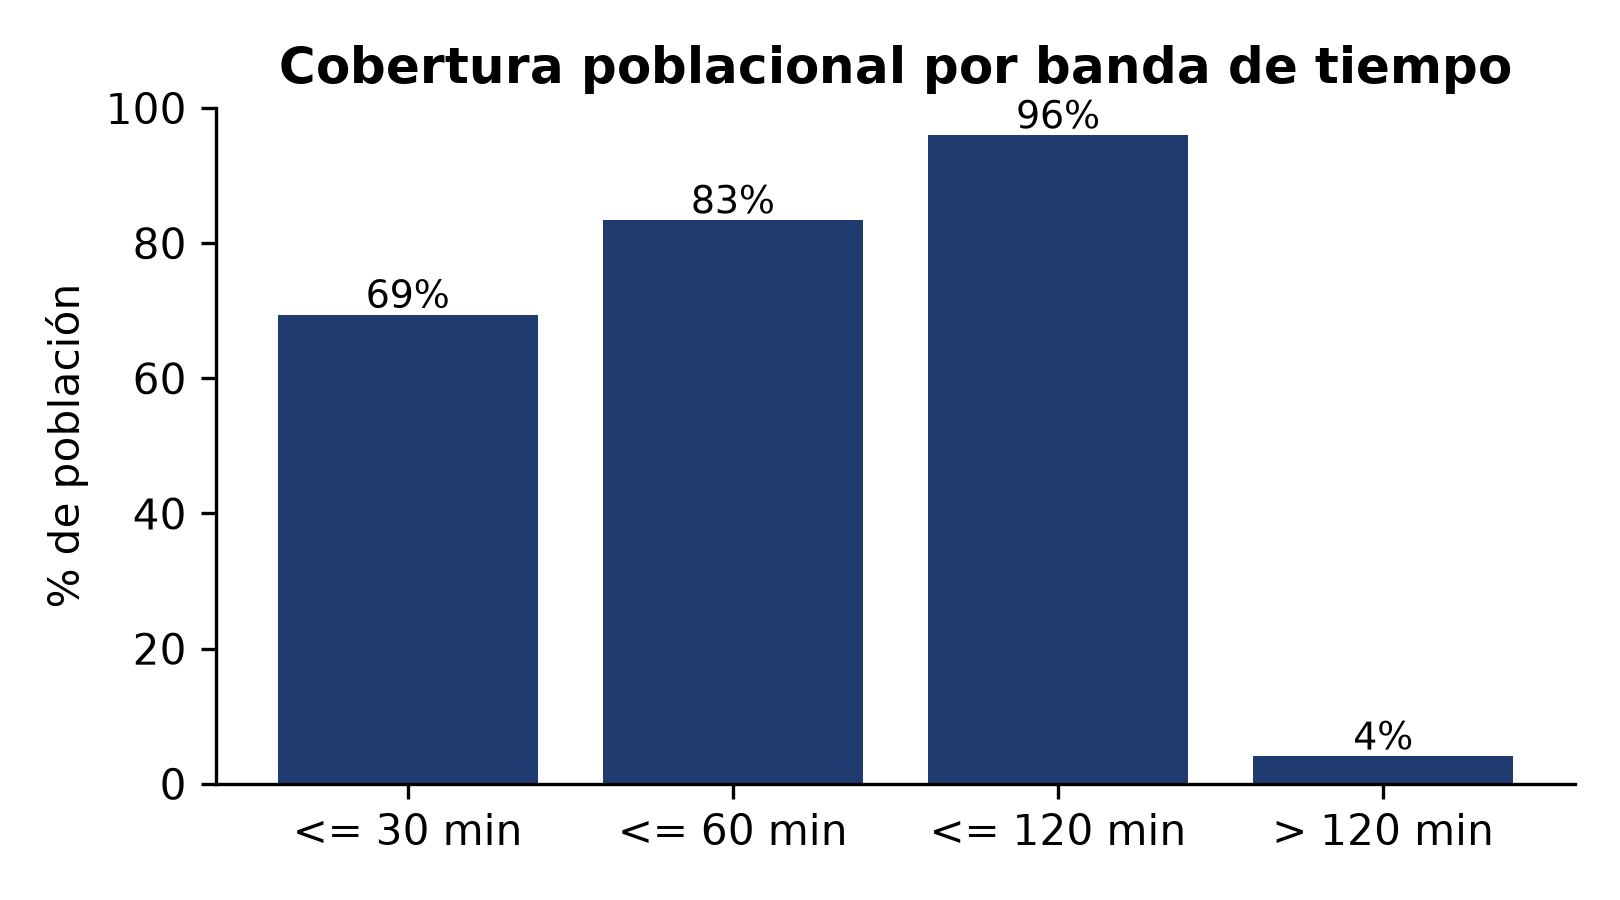
\includegraphics[width=0.49\linewidth]{fig_cobertura.png}\hfill
  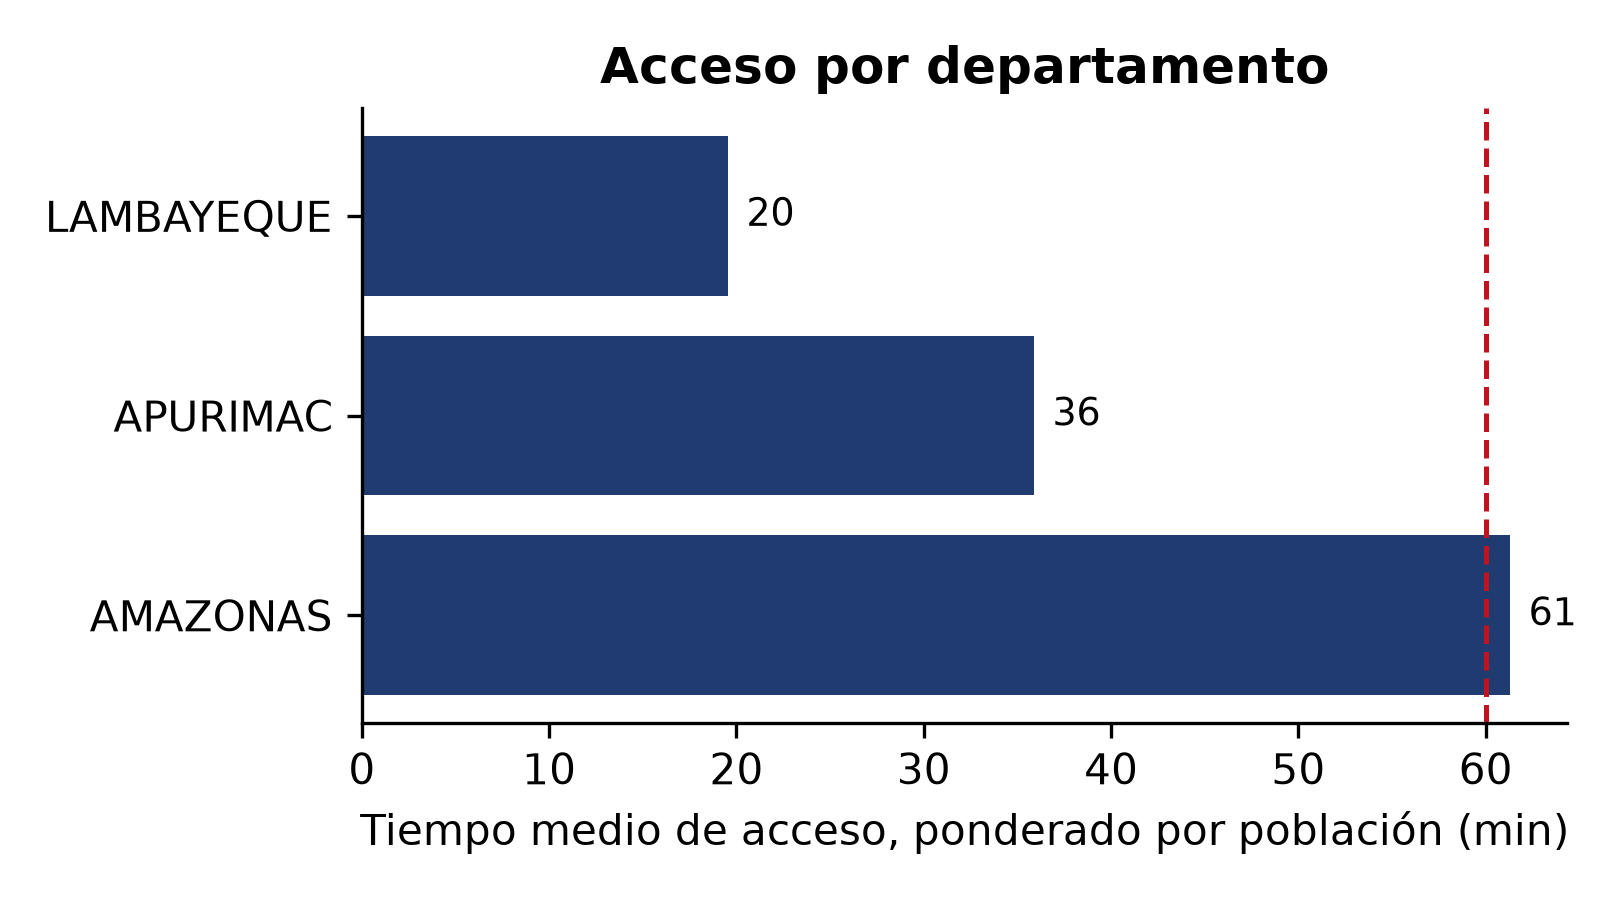
\includegraphics[width=0.49\linewidth]{fig_departamento.png}
  \caption{Izquierda: cobertura poblacional por banda de tiempo. Derecha: tiempo
  medio de acceso por departamento.}
  \label{fig:cobertura}
\end{figure}

\begin{figure}[H]
  \centering
  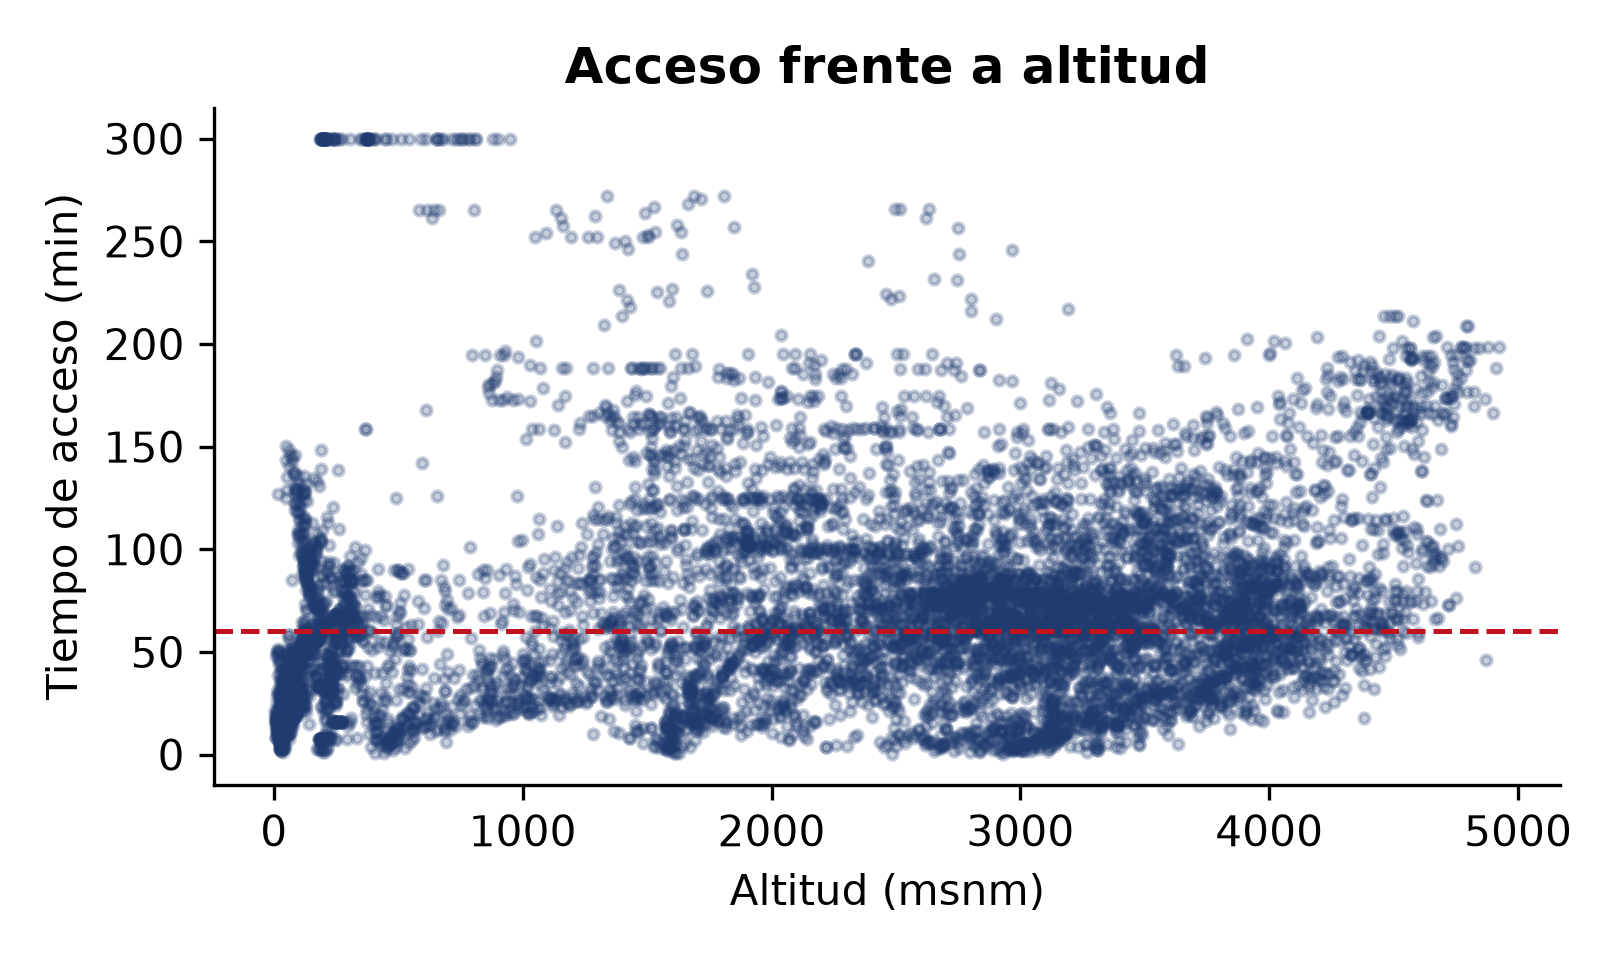
\includegraphics[width=0.72\linewidth]{fig_altitud.png}
  \caption{Tiempo de acceso frente a altitud del centro poblado.}
  \label{fig:altitud}
\end{figure}

\tab{tab_cobertura.tex}
\tab{tab_departamento.tex}
\tab{tab_distritos_peores.tex}

\paragraph{S\'intesis num\'erica} (perfil conducci\'on, ponderado por poblaci\'on;
fuente: \texttt{data/outputs/summary.json}).
\begin{itemize}
  \item Poblaci\'on del \'ambito: \num{1982403} habitantes en \num{8781} centros
        poblados; \num{39} establecimientos resolutivos.
  \item \textbf{Fuera de la hora dorada: \SI{16.6}{\percent}} de la poblaci\'on
        (\SI{4.1}{\percent} a m\'as de 120 min). Cobertura acumulada:
        \SI{69.4}{\percent} a \SI{30}{min}, \SI{83.4}{\percent} a \SI{60}{min}.
  \item Tiempo medio ponderado \SI{30.9}{min}; mediana de centros poblados
        \SI{63.8}{min}: la poblaci\'on se concentra cerca de los hospitales,
        pero la mayor\'ia de localidades peque\~nas queda lejos.
  \item \textbf{Gini de acceso: \num{0.66}}.
  \item Urbano vs rural: \SI{11.4}{min} vs \SI{62.9}{min}.
  \item Por departamento: Lambayeque \SI{19.5}{min} (\SI{8.1}{\percent} fuera),
        Apur\'imac \SI{35.9}{min} (\SI{25.4}{\percent}), Amazonas
        \SI{61.3}{min} (\SI{34.2}{\percent}).
  \item Tercil de altitud (bajo/medio/alto): \SIlist{25.2;39.9;57.4}{min}.
  \item \textbf{Cuartil de pobreza distrital}: del menos al m\'as pobre,
        \SIlist{15.5;47.0;58.1;113.2}{min}. Correlaci\'on de $t_i$ con \% de
        pobreza $r=\num{0.35}$; con IDH $r=\num{-0.38}$.
  \item Comparaci\'on de perfiles: \SI{30.9}{min} en coche frente a
        \SI{393}{min} a pie (media ponderada) --- caminar no es una alternativa
        viable para la emergencia en este territorio.
\end{itemize}

\section{Discusi\'on}
El acceso es marcadamente desigual: la poblaci\'on urbana costera est\'a casi
siempre dentro de la hora dorada, mientras que en la sierra y la selva la
mediana de los centros poblados supera ese umbral. La brecha se alinea con la
pobreza distrital, lo que sugiere que la carencia de acceso a emergencias
refuerza desventajas preexistentes. La altitud act\'ua como proxy de la
dificultad de la red vial.

\section{Limitaciones}
\begin{itemize}
  \item Modelo est\'atico: sin tr\'afico, clima, estado del firme ni
        estacionalidad (crecidas amaz\'onicas).
  \item El \emph{fallback} y el perfil peatonal son cotas inferiores.
  \item La cobertura de OSM es menor en la selva; algunas v\'ias no est\'an
        mapeadas.
  \item La poblaci\'on de centros poblados es del Censo 2017; no capta
        migraci\'on reciente.
  \item Se consideran solo establecimientos dentro de los tres departamentos;
        se ignoran efectos de borde con regiones vecinas.
\end{itemize}

\section{Conclusiones}
Cerca de \num{330} mil personas (\SI{16.6}{\percent}) de Lambayeque, Apur\'imac y
Amazonas no pueden alcanzar un establecimiento de salud resolutivo dentro de la
hora dorada por carretera, y la carencia se concentra en la selva, en la altura
y --- de forma marcada --- en los distritos m\'as pobres, que tardan del orden de
siete veces m\'as que los menos pobres. El elevado coeficiente de Gini
(\num{0.66}) confirma que el problema no es un d\'eficit medio sino una
distribuci\'on muy desigual: bastar\'ia elevar a categor\'ia resolutiva unos
pocos establecimientos bien ubicados en la sierra y la selva para reducir de
forma apreciable la poblaci\'on fuera de cobertura, hip\'otesis que el simulador
del panel permite explorar.

\section*{Reproducibilidad}
C\'odigo y datos: \url{https://github.com/karelysscs/Practica_2_Data_Science}.
Ejecutar en orden \texttt{python -m src.phase1\_data}, \texttt{src.phase2\_routing},
\texttt{src.phase3\_metrics}, \texttt{src.figures}; dashboard con
\texttt{streamlit run app.py}.

\begin{thebibliography}{9}
\bibitem{golden} Lerner, E.B.; Moscati, R.M. (2001). The Golden Hour:
  scientific fact or medical urban legend? \emph{Acad. Emerg. Med.} 8(7).
\bibitem{osrm} Luxen, D.; Vetter, C. (2011). Real-time routing with
  OpenStreetMap data. \emph{ACM SIGSPATIAL GIS}.
\bibitem{renipress} SUSALUD. Registro Nacional de IPRESS (RENIPRESS), 2026.
\bibitem{inei} INEI. Censos Nacionales 2017: XII de Poblaci\'on y VII de
  Vivienda --- Centros Poblados.
\end{thebibliography}

\end{document}
